\documentclass[10pt]{article}
\usepackage[margin=2.2cm]{geometry}
\usepackage{booktabs,longtable,graphicx,array,xcolor,framed}
\usepackage[hidelinks]{hyperref}
\setlength{\tabcolsep}{4pt}
\title{Tuning report: tropical / SCC}
\date{2026-10-22T19:17:34}
\begin{document}
\maketitle

\section{Decision}
Approving freezes
\texttt{fishr.lambda} $=$ 1000 into every cell of the grid (frozen hash \texttt{d8981f9390da}).
The experiment YAML has
\texttt{fishr.lambda} $=$ 1000 for this campaign.
\texttt{frozen.yaml} is currently unapproved with \{'fishr.lambda': 1000.0\}.

\paragraph{Selection rule.} The candidate with the lowest mean \texttt{id\_val\_loss} wins, averaged over 6 cell(s) and 2 tuning seed(s) each (global seed 1000, disjoint from the grid's 0), across 4 candidates. A candidate with a missing or diverged run is not eligible.

\begin{framed}
\noindent\textbf{Verdict: \textcolor{orange!85!black}{REVIEW}}
\begin{itemize}\setlength\itemsep{0pt}
\item \textbf{review}: the winner is not distinguishable from fishr.lambda=100: the paired gap's 95\% CI is [-6.06e-05, 6.91e-05]
\item \textbf{review}: fishr.lambda=10: fishr.lambda * fishr\_penalty\_final is 0.0014 of id\_val\_loss (median over runs); the term barely enters the loss
\item \textbf{review}: 12 of 12 winner runs reached their best id\_val\_loss at the last logged epoch: the search budget may be too short to rank candidates
\item \textbf{review}: 12 of 12 winner runs picked their last epoch (best\_epoch = 19): still improving when the search budget ran out, so candidates were ranked before converging
\item \textbf{info}: the search ran with optim.epochs=20; the grid runs with optim.epochs=100
\item \textbf{info}: devices: cuda:0
\end{itemize}
\end{framed}
\noindent\textbf{block}: do not approve; fix the search and re-run it. \textbf{review}: read the sections below before approving. \textbf{info}: context only.

\section{Search setup}
\begin{itemize}\setlength\itemsep{0pt}
\item \texttt{fishr.lambda} $\in \{$10, 100, 1000, 1e+04$\}$
\item Cells trained (\texttt{tune.only} \{'objective': 'fishr'\}):
\begin{itemize}\setlength\itemsep{0pt}
\item \texttt{model\_type=vanilla head=seq2seq objective=fishr}
\item \texttt{model\_type=vanilla head=pointer objective=fishr}
\item \texttt{model\_type=adaptive head=seq2seq objective=fishr}
\item \texttt{model\_type=adaptive head=pointer objective=fishr}
\item \texttt{model\_type=tropical head=seq2seq objective=fishr}
\item \texttt{model\_type=tropical head=pointer objective=fishr}
\end{itemize}
\item Search-only overrides (never frozen): \texttt{\{'optim': \{'epochs': 20\}\}}. The chosen value was ranked under this budget, not the grid's.
\end{itemize}

\section{Candidates}
\autoref{tab:candidates} ranks the candidates on \texttt{id\_val\_loss} (lower is better); \autoref{fig:sensitivity} plots them.
Candidates share seeds, so \autoref{tab:gaps} compares each with the winner run by run (same cell, same seed).

{\small
\begin{longtable}{rlrrrlrll}
\caption{Every candidate: rank, runs stored/expected, diverged, mean with 95\% bootstrap CI, SD and range over all its runs.}\label{tab:candidates}\\
\toprule
\# & \texttt{fishr.lambda} & runs & div. & mean & 95\% CI & SD & range & \\
\midrule
\endhead
3 & 10 & 12/12 & 0 & 0.003319 & [0.00307, 0.00362] & $5.17\times10^{-4}$ & [0.00279, 0.00438] & \\
2 & 100 & 12/12 & 0 & 0.003284 & [0.00304, 0.00354] & $4.80\times10^{-4}$ & [0.00263, 0.00421] & \\
1 & 1000 & 12/12 & 0 & 0.003281 & [0.00302, 0.00357] & $5.19\times10^{-4}$ & [0.00256, 0.00436] & \textbf{selected}\\
4 & 1e+04 & 12/12 & 0 & 0.00341 & [0.00317, 0.00369] & $4.78\times10^{-4}$ & [0.00295, 0.00442] & \\
\bottomrule
\end{longtable}
}

{\small
\begin{longtable}{lrrlrrrl}
\caption{Each candidate minus the winner on the runs they share, signed so a positive gap is worse than the winner. Worse/better/equal count the runs; $p$ is a two-sided sign test.}\label{tab:gaps}\\
\toprule
candidate & $n$ & gap & 95\% CI & worse & better & equal & $p$\\
\midrule
\endhead
\texttt{fishr.lambda=10} & 12 & $3.875\times10^{-5}$ & [$-1.19\times10^{-5}$, $9.90\times10^{-5}$] & 7 & 5 & 0 & 0.7744\\
\texttt{fishr.lambda=100} & 12 & $3.363\times10^{-6}$ & [$-6.06\times10^{-5}$, $6.91\times10^{-5}$] & 7 & 5 & 0 & 0.7744\\
\texttt{fishr.lambda=10000} & 12 & $1.298\times10^{-4}$ & [$6.44\times10^{-5}$, $2.07\times10^{-4}$] & 10 & 2 & 0 & 0.0386\\
\bottomrule
\end{longtable}
}

\begin{figure}[htbp]
\centering
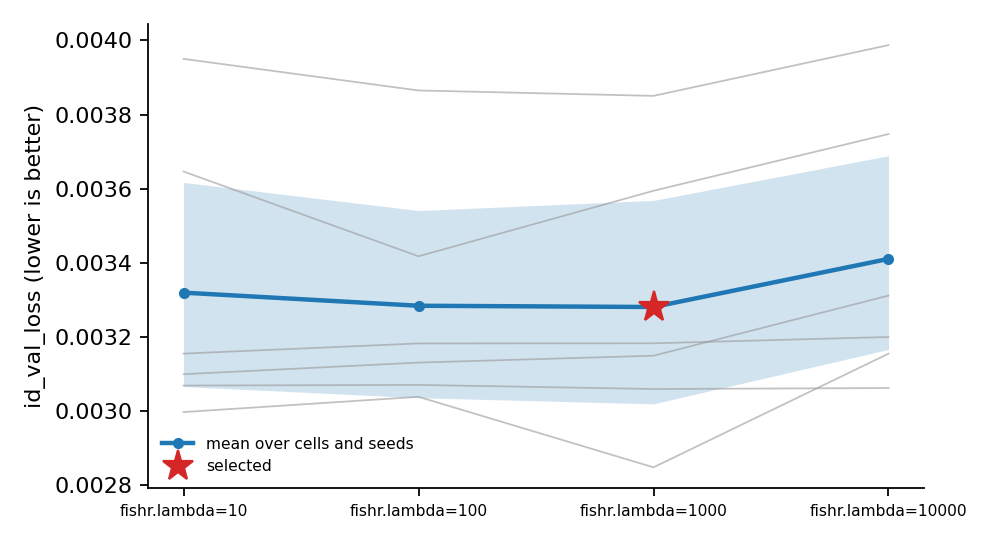
\includegraphics[width=\textwidth]{tune_sensitivity.png}
\caption{\texttt{id\_val\_loss} per candidate: the mean over every run with a 95\% bootstrap CI (blue), each cell's seed-mean (grey), the selected candidate (red star).}
\label{fig:sensitivity}
\end{figure}

\section{Per cell}
One value is frozen for every cell, chosen by the mean over cells. \autoref{fig:cells} shows whether the winner is best in each cell or is carried by a few of them.
\begin{figure}[htbp]
\centering
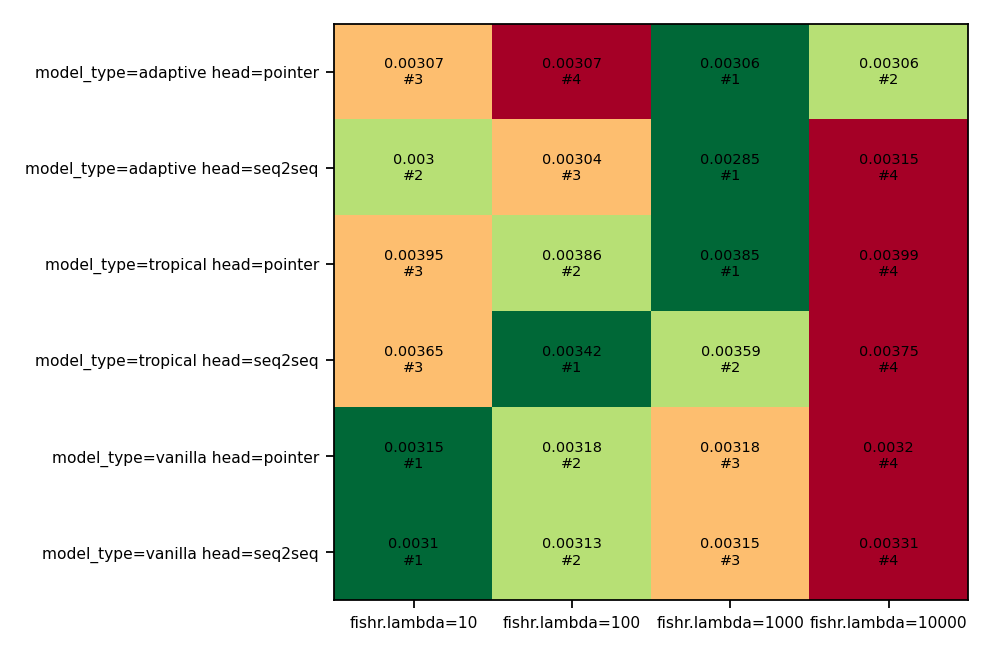
\includegraphics[width=\textwidth]{tune_cells.png}
\caption{Each cell's seed-mean \texttt{id\_val\_loss} per candidate, with its rank within the cell (\#1 is best; green is better).}
\label{fig:cells}
\end{figure}
{\small
\begin{longtable}{ll}
\caption{The best candidate in each cell.}\label{tab:cells}\\
\toprule
cell & best\\
\midrule
\endhead
\texttt{model\_type=adaptive head=pointer} & fishr.lambda=1000\\
\texttt{model\_type=adaptive head=seq2seq} & fishr.lambda=1000\\
\texttt{model\_type=tropical head=pointer} & fishr.lambda=1000\\
\texttt{model\_type=tropical head=seq2seq} & fishr.lambda=100\\
\texttt{model\_type=vanilla head=pointer} & fishr.lambda=10\\
\texttt{model\_type=vanilla head=seq2seq} & fishr.lambda=10\\
\bottomrule
\end{longtable}
}

\section{Other training-distribution metrics}
Not used for selection; shown so a winner that trades them away is visible.
{\small
\begin{longtable}{lrrrr}
\caption{Mean of every other in-distribution metric per candidate.}\label{tab:open}\\
\toprule
candidate & \texttt{id\_f1} & \texttt{id\_exact} & \texttt{fishr\_penalty\_final} & \texttt{best\_epoch}\\
\midrule
\endhead
fishr.lambda=10 & 0.996 & 0.979 & $1.04\times10^{-6}$ & 19\\
fishr.lambda=100 & 0.996 & 0.979 & $4.75\times10^{-7}$ & 19\\
\textbf{fishr.lambda=1000} & 0.996 & 0.979 & $1.29\times10^{-7}$ & 19\\
fishr.lambda=10000 & 0.996 & 0.979 & $4.12\times10^{-8}$ & 19\\
\bottomrule
\end{longtable}
}

\section{Training curves}
The mean over every cell and seed of each candidate; the selected candidate in bold red.
\begin{figure}[htbp]
\centering
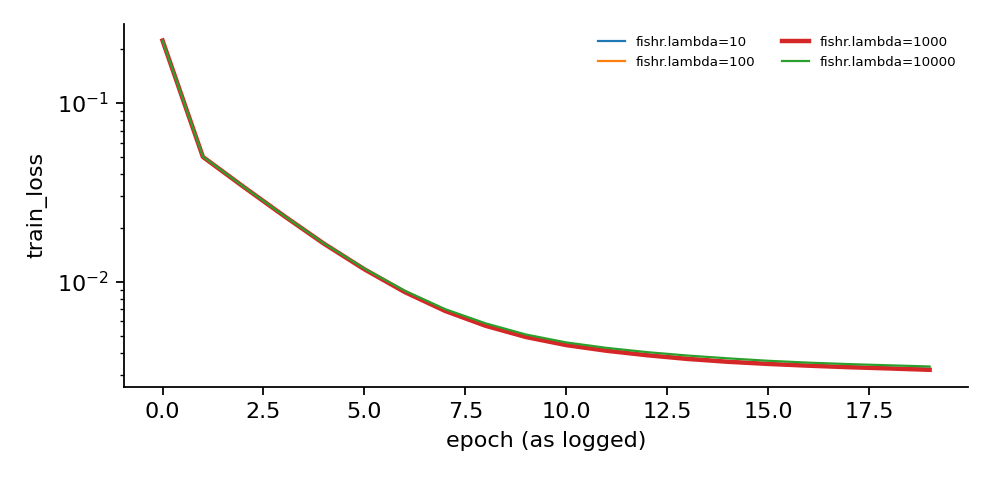
\includegraphics[width=\textwidth]{tune_curve_train_loss.png}
\caption{\texttt{train\_loss} per candidate.}
\label{fig:curve-train_loss}
\end{figure}
\begin{figure}[htbp]
\centering
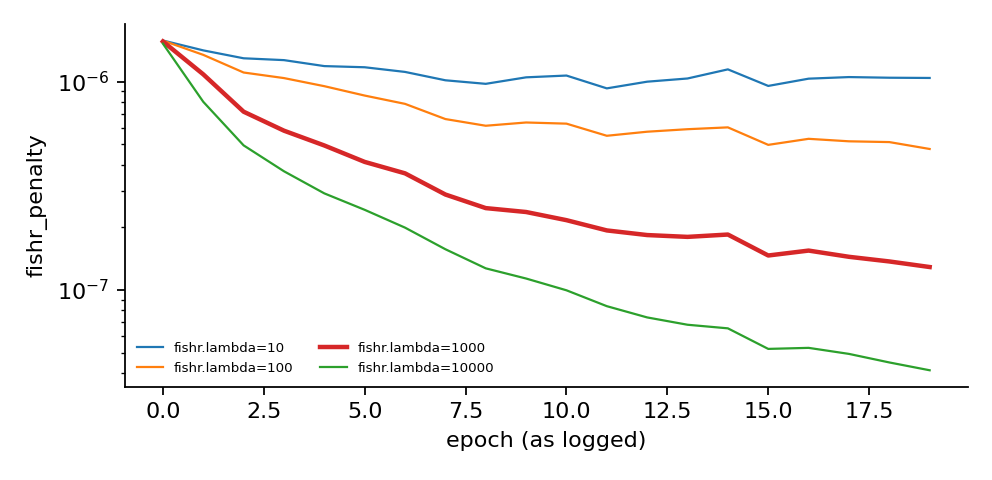
\includegraphics[width=\textwidth]{tune_curve_fishr_penalty.png}
\caption{\texttt{fishr\_penalty} per candidate.}
\label{fig:curve-fishr_penalty}
\end{figure}
\begin{figure}[htbp]
\centering
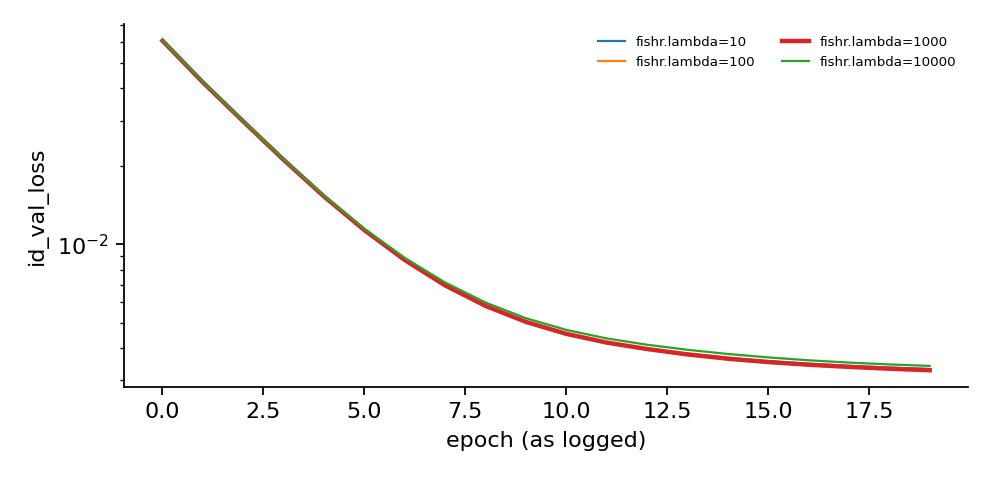
\includegraphics[width=\textwidth]{tune_curve_id_val_loss.png}
\caption{\texttt{id\_val\_loss} per candidate.}
\label{fig:curve-id_val_loss}
\end{figure}

\clearpage
\section{Provenance}
{\small
\begin{longtable}{llrrll}
\caption{Each candidate's runs: base hash, runs, total wall time, commits (+ marks a dirty tree), torch.}\label{tab:provenance}\\
\toprule
candidate & hash & runs & wall (s) & commit & torch\\
\midrule
\endhead
fishr.lambda=10 & \texttt{b7150148661b} & 12 & 3.51e+04 & \texttt{e5ccce8034} & 2.8.0+cu128\\
fishr.lambda=100 & \texttt{7984c1850aea} & 12 & 2.41e+04 & \texttt{e5ccce8034} & 2.8.0+cu128\\
fishr.lambda=1000 & \texttt{52ab10df6885} & 12 & 2.04e+04 & \texttt{e5ccce8034} & 2.8.0+cu128\\
fishr.lambda=10000 & \texttt{5a197ec9fc42} & 12 & 3.78e+04 & \texttt{e5ccce8034} & 2.8.0+cu128\\
\bottomrule
\end{longtable}
}
\noindent Store: \texttt{campaigns/tropical/SCC/tune/results}.\\
Rebuild: \texttt{expkit tune-report --config configs/tropical.yaml --profile SCC}\\
Approve: \texttt{expkit approve --config configs/tropical.yaml --profile SCC}

\paragraph{The base the grid would run with.}
{\footnotesize
\begin{verbatim}
task:
  name: SCCDataset
  value_range: 0.001
  target_range: null
  weight_range: null
  adversarial_range: null
  noise_prob: 0.0
data:
  train_lengths:
  - 4
  - 5
  - 6
  - 7
  - 8
  ood_lengths:
  - 12
  - 16
  ood_value_range: 0.1
  ood_noise_range: null
  ood_noise_prob: 0.5
  n_per_length: 20000
  n_eval_per_length: 2000
  curve_eval_limit: 256
model:
  d_model: 64
  n_heads: 2
  num_layers: 1
  dropout: 0.0
  tropical_impl: legacy
optim:
  lr: 0.0001
  epochs: 100
  batch_size: 8
  eval_batch_size: 8
fishr:
  lambda: 1000.0
  ema: 0.95
  anneal_iters: 1500
  reset_optimizer: true
\end{verbatim}
}

\clearpage
\appendix
\section{Sealed: OOD and test metrics}
\textbf{Read this only after deciding.} These were recorded by the tuning runs but never consulted by the selection. Choosing a value because it looks better here would tune on the test distribution.
{\small
\begin{longtable}{lrrrrrrrrrr}
\caption{Mean of every OOD or test metric per candidate.}\label{tab:sealed}\\
\toprule
candidate & \rotatebox{70}{\texttt{ood\_len\_f1}} & \rotatebox{70}{\texttt{ood\_len\_exact}} & \rotatebox{70}{\texttt{ood\_val\_f1}} & \rotatebox{70}{\texttt{ood\_val\_exact}} & \rotatebox{70}{\texttt{ood\_noise\_f1}} & \rotatebox{70}{\texttt{ood\_noise\_exact}} & \rotatebox{70}{\texttt{ood\_len\_f1\_L12}} & \rotatebox{70}{\texttt{ood\_len\_exact\_L12}} & \rotatebox{70}{\texttt{ood\_len\_f1\_L16}} & \rotatebox{70}{\texttt{ood\_len\_exact\_L16}}\\
\midrule
\endhead
fishr.lambda=10 & 0.649 & 0.165 & 0.965 & 0.87 & 0.722 & 0.321 & 0.79 & 0.31 & 0.576 & 0.0204\\
fishr.lambda=100 & 0.644 & 0.135 & 0.965 & 0.87 & 0.706 & 0.312 & 0.784 & 0.249 & 0.571 & 0.0218\\
\textbf{fishr.lambda=1000} & 0.652 & 0.131 & 0.965 & 0.868 & 0.707 & 0.321 & 0.782 & 0.24 & 0.583 & 0.0232\\
fishr.lambda=10000 & 0.679 & 0.227 & 0.965 & 0.869 & 0.716 & 0.336 & 0.782 & 0.371 & 0.622 & 0.0834\\
\bottomrule
\end{longtable}
}
\end{document}